% status: 98
% chapter: REST


\def\paperstatus{100} % a number from 0-100 indicating your status. 100
                % means completed
\def\paperchapter{REST} % This section is typically a single keyword. from
                   % a small list. Consult with theinstructors about
                   % yours. They typically fill it out once your first
                   % text has been reviewed.
\def\hid{hid-sp18-523, hid-sp18-520} % all hids of the authors of this
                                % paper. The paper must only be in one
                                % authors directory and all other
                                % authors contribute to it in that
                                % directory. That authors hid must be
                                % listed first
\def\volume{9} % the volume of the proceedings in which this paper is to
           % be included

\def\locator{\hid, Volume: \volume, Chapter: \paperchapter, 
Status: \paperstatus. \newline}

\title{REST Service Framework with SciKit Learn Algorithms}

\author{Arijit Sinha}
\affiliation{%
  \institution{Indiana University}
  \city{Bloomington} 
  \state{IN} 
  \postcode{47408}
  \country{USA}}
\email{arisinha@iu.edu}

\author{Ritesh Tandon}
\affiliation{%
  \institution{Indiana University}
  \city{Bloomington} 
  \state{IN} 
  \postcode{47408}
  \country{USA}}
\email{ritandon@iu.edu}

% The default list of authors is too long for headers}
\renewcommand{\shortauthors}{G. v. Laszewski}


\begin{abstract}
In current world, data is getting generated and stored with different 
storage systems. We need to use this data for a better understanding, analyze 
and can estimate the future scenarios with certain probability. There are many 
algorithms, which have developed and implemented for providing better accuracy 
on the future scenarios.
\end{abstract}

\keywords{\locator\ REST, scikit learn, linear, decision tree, 
random forest, algorithm, Machine, learning}


\maketitle

\section{Introduction}

Scikit learn is a library created under machine learning algorithms, 
which uses different datasets gathered over years to learn and predicts 
future scenarios. Supervised and unsupervised learning can differentiation 
conducted for learning variety of dataset.

Supervised algorithms are on the dataset, which has the target variable, which 
need to be predicted or estimated. This datasets can be acted with below 
different approaches

Classification is based on the classes and the labeled data, we need to predict
 the unlabeled data.

Regression is based on the continuous variable or data, we need to predict the 
future state of data is known as regression

Unsupervised algorithms are on the dataset, where we donot see the 
target variable for prediction, we learn its behavior set of vector input 
variable to identify the clustering group of similar behavior data or sample
~\cite{sckitml}
Kaggle is a known location for different kind of datasets gathered by various 
institutes across globe.

\section{Scope of work}

Below are the 3 algorithm from Scikit learn
\begin{itemize}
\item Implement Linear Regression
\item Implement Boosted Decision
\item Implement Hyper-tuned Boosted Decision
\end{itemize}

\section{Reason}

We are planning to use Regression learning algorithm because the target 
variable is numerical and continuous in nature. We will be creating ML 
pipeline using linear, regularized linear, tree and forest learning algorithm.
 We will compare and evaluate different models based on RMSE of learning 
algorithm.
~\cite{sckitml}

\section{Technology Stack}

Python will be used for Data loading, preprocessing and cleaning. Using 
Scikit learn library, we will implement variety of algorithms to conduct 
above process and finally will predict the sale price of its products.

REST services has been implemented to provide a prediction of price of the 
products:

\begin{itemize}
	\item REST data preprocessing: It will be the service, which does 
the data processing 
	with removal or imputing the data with mean or median. Removal of 
the columns which doesn’t any correlation with target variable
	\item REST data prediction: it will be the service, which will 
do multiple predictions using multiple algorithms as below
	
	\item Rest API with Linear Regression – Display the outcome 
of product and predicted price
	\item Rest API with Boosted Decision – Display the outcome of 
product and predicted price
	\item Rest API with Hyper-tuned Boosted Decision – Display the 
outcome of product and predicted price
\end{itemize}

Cloud technology utilized will be Microsoft Azure, AWS, it has been 
implemented at Local machine and Docker.

We have acquired the dataset from Kaggle and read the data dictionary details 
on different websites which includes below describes attributes. We have 14204 
instances and 13 attributes in the dataset, which will be spitted into 
Training and Test Data set. This dataset is available on public websites

BigMart Dataset, With this dataset, we will predict the sale price of 
various products based on the learning of historical data in the datasets 
using different algorithm. The dataset has various data with respect to
\begin{itemize}
\item $Item_Fat_Content$
\item $Item_Identifier$
\item $Item_MRP$
\item $Item_Outlet_Sales$
\item $Item_Type$
\item $Item_Visibility$
\item $Item_Weight$
\item $Outlet_Establishment_Year$
\item $Outlet_Identifier$
\item $Outlet_Location_Type$
\item $Outlet_Size$
\item $Outlet_Type$
\item source
\end{itemize}
~\cite{kaggleds}


\section{Dataset Details}
It has following 12 attributes with continuous and categorical values 
with Unique Values
\begin{itemize}
\item $Item_Fat_Content has 5 unique values$
\item $Item_Identifier has 1559 unique values$
\item $Item_MRP has 8052 unique values$
\item $Item_Outlet_Sales has 3494 unique values$
\item $Item_Type has 16 unique values$
\item $Item_Visibility has 13006 unique values$
\item $Item_Weight has 416 unique values$
\item $Outlet_Establishment_Year has 9unique values$
\item $Outlet_Identifier has 10 unique values$
\item $Outlet_Location_Type has 3 unique values$
\item $Outlet_Size has 4 unique values$
\item $Outlet_Type has 4 unique values$
\end{itemize}


\section{Data Visualization}
Histogram shows the distribution of data of different variables 

Plotting Histogram from Dataset

\begin{figure}[pic1]
\centering
\includegraphics[width=\columnwidth]{Images/mlstudio/
HistrogramofImpAttributes.png}
\caption{HistrogramofImpAttributes}
\label{fig:HistrogramofImpAttributes}
\end{figure}

Correlation plot informs about the relation between variables 
\begin{figure}[pic2]
\centering
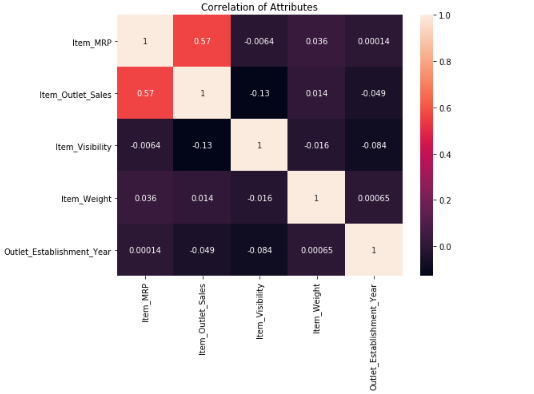
\includegraphics[width=\columnwidth]{Images/mlstudio/Correlation.png}
\caption{Correlation}\label{fig:Correlation}
\end{figure}

\section{Data Exploration}
Analyzed and plotted the categorical and continuous feature summaries to 
see which feature is 
closely related with target variable. This helped us with deciding which 
feature are influencing 
the prediction.

\section{Data Preprocessing}
\begin{itemize}
\item Missing values (2439) of item weight is replaced with mean.
\item Missing values (4016) of outlet size observations, which been 
replaced with mode.
\end{itemize}


\section{Azure ML Studio}
Azure ML studio provides the GUI interface for creating the Machine 
Learning Train models and Predictions. It provides a provision to integrate 
with Azure Cloud and expose the Web Services

\subsection{Train Model with Azure}
Created on Azure ML Studio, 3 Learning Algorithms used
\begin{itemize}
\item Boosted Decision Tree
\item Linear Regression
\item HyperTuned Boosted Decision Tree
\end{itemize}

From the RMSE results, Hyper-tuned Boosted Decision Tree has provided better 
results.

\begin{figure}[pic3]
\centering
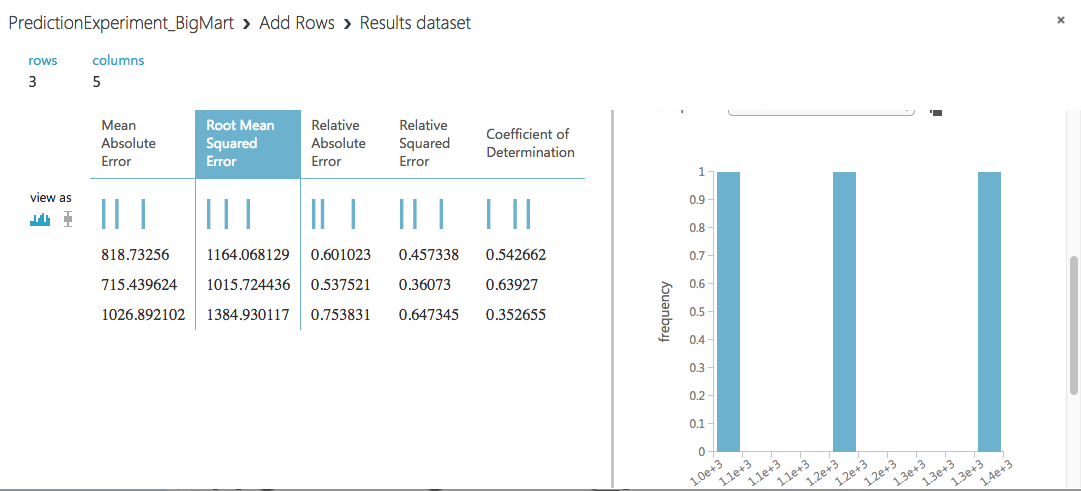
\includegraphics[width=\columnwidth]{Images/mlstudio/RMSEComparison.png}
\caption{RMSEComparison.png}\label{fig:RMSEComparison}
\end{figure}

\begin{figure}[pic4]
\centering
\includegraphics[width=\columnwidth]{Images/mlstudio/
RMSEComparisionBetweenHypertune.png}
\caption{RMSEComparisionBetweenHypertune.png}
\label{fig:RMSEComparisionBetweenHypertune}
\end{figure}

\subsection{Predictive Model}
Update the Trained model with Test dataset for predicting the Item Outlet 
Sales data. Verified and updated the data cleaning process which we have 
implemented for Train dataset. After converting the categorical data with 
indicators, we can apply the trained model.

Created predictive model using the above Hyper-tuned Boosted Decision Tree.

From the score function, have extracted only 2 columns
\begin{itemize}
\item Item Identifer
\item Item Outlet Sales
\end{itemize}

Create the Web service input and Web service Output.

\begin{figure}[pic5]
\centering
\includegraphics[width=\columnwidth]{Images/mlstudio/
PredictionOutputfromModel.png}
\caption{PredictionOutputfromModel.png}
\label{fig:PredictionOutputfromModel}
\end{figure}

\subsection{Web Service Deployment}
Once the Prediction model has been executed successfully, it can be deployed 
as web service from Azure ML Studio.

It will generate the API key, which will be used for Azure Cloud deployment.

\begin{figure}[pic6]
\centering
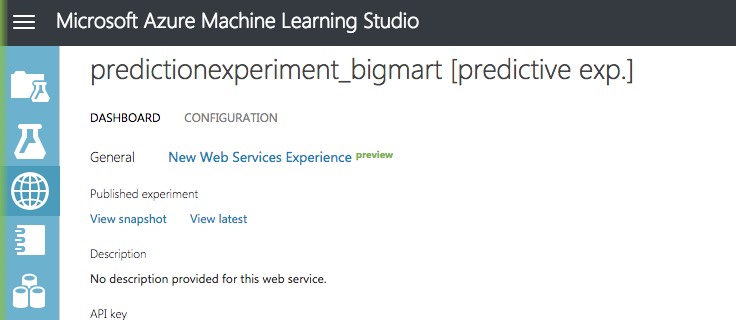
\includegraphics[width=\columnwidth]{Images/mlstudio/Webservicedeploy.png}
\caption{Webservicedeploy.png}
\label{fig:Webservicedeploy}
\end{figure}

It will provide an option to Test web service locally with below options
\begin{itemize}
\item Click on Test button enabled at the bottom of the screen
\item Download the CSV file from the tool to test the Web API 
with prediction model.
\end{itemize}

\subsection{Azure Cloud deployment}
Once the Web Service is created locally, It will create a hyper link with 
name of the web service. 
Click on the hyperlink generated on the Name of web service.

It will open the web service dashboard for configuration and setup the 
consumption process with Azure cloud.

It will provide the test tab on the dashboard, where we can provide the 
inputs and get the prediction values once clicked on Test Request response 
button.

This step will assure that, the web services are working as expected.

\begin{figure}[pic7]
\centering
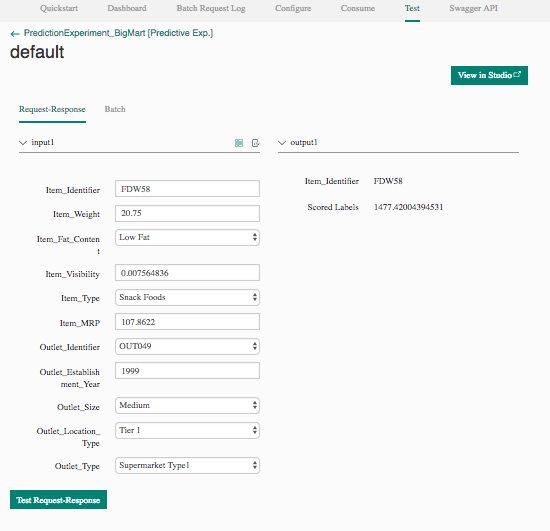
\includegraphics[width=\columnwidth]{Images/mlstudio/Webserviceconf.png}
\caption{Webserviceconf}\label{fig:Webserviceconf}
\end{figure}

After clicking consume tab from Dashboard, It will display option for 
Response Request Web Template link.

Copy the request response link generated on the page.

Once clicked on the link, it will redirect to Azure cloud configuration 
using Response Request Web application.

Azure ML Request, Response Service Web App
In Azure cloud, it need to created as

\begin{itemize}
\item Create the request response service web app
\item Create Resource Group
\item Add Model Management services
\item Click on the URL link generated under resource group
\item Update the Settings with API POST URL
\item Update the API key generated from Web service from Azure ML studio.
\end{itemize}

Expose the Web Service from Azure cloud

Click on the below link to access the prediction web service  
https://predictbigmart.azurewebsites.net/

Entered the values used to for testing locally, the amount should 
match so as to see if the service is functioning as expected.

\begin{figure}[pic8]
\centering
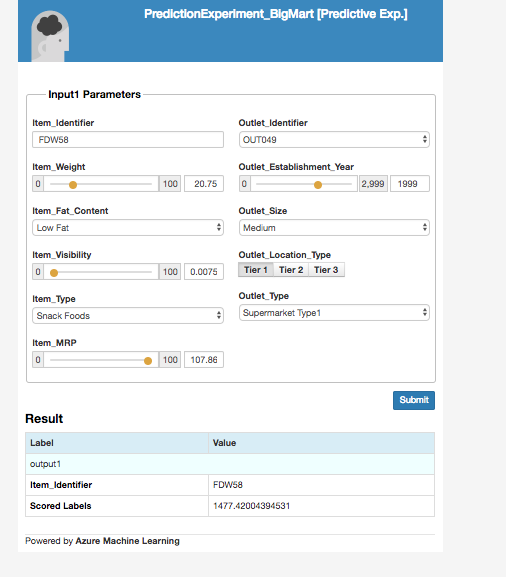
\includegraphics[width=\columnwidth]{Images/mlstudio/WebService.png}
\caption{WebService}\label{fig:WebService}
\end{figure}

Batch Mode for Web Service Execution
Download the CSV generated from Azure ML Studio 
\begin{itemize}
\item Open the CSV, it will be open with Web API built in
\item Use Sample data link on the API
\item Select the range of columns and provide as input to API
\item Select the cell from where the prediction values needs to be displayed.
\item Click on Prediction button.
It will generate the prediction values for all the selected Input entries 
with Item Identifiers.
\end{itemize}

\begin{figure}[pic9]
\centering
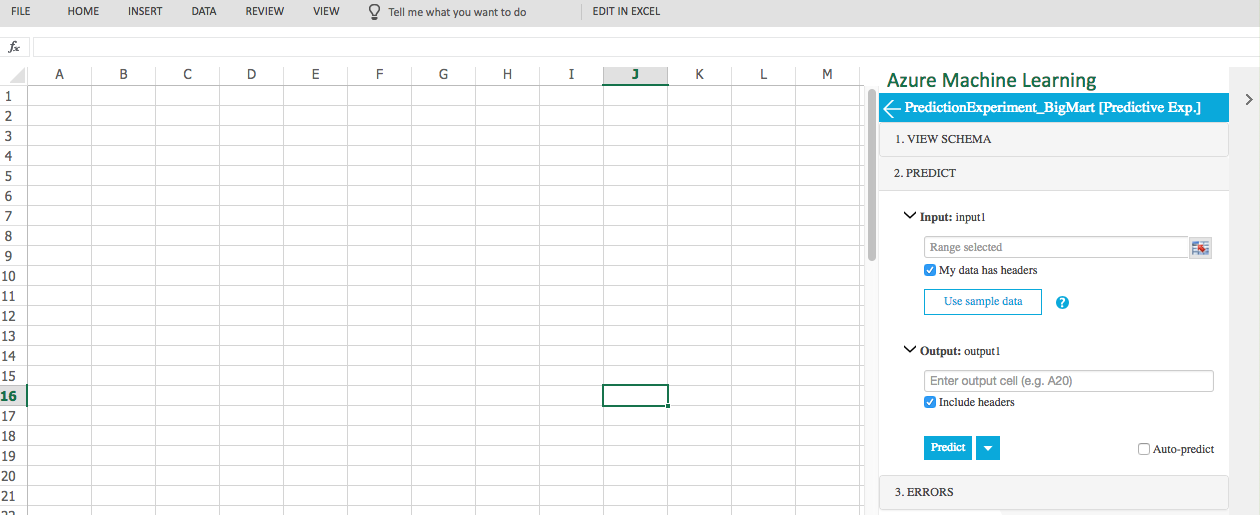
\includegraphics[width=\columnwidth]{Images/mlstudio/csvscreenshot.png}
\caption{csvscreenshot}\label{fig:csvscreenshot}
\end{figure}

\subsection{Azure ML Studio with Challenge}
With Azure ML Studio, downloading code is not provided as an option.

\section{Azure with Notebook Instance}

On Azure ML Studio, there is another option of executing the Machine 
learning Algorithms. Its known as Notebook Instance, in this section, 
there can be a Jupyter notebook created and executed with the Train Model, 
followed by prediction.Captured the time of execution on the same with 15.2 ms 
for overall batch prediction. With Model, the computation time is 1.95 ms

\begin{figure}[pic9]
\centering
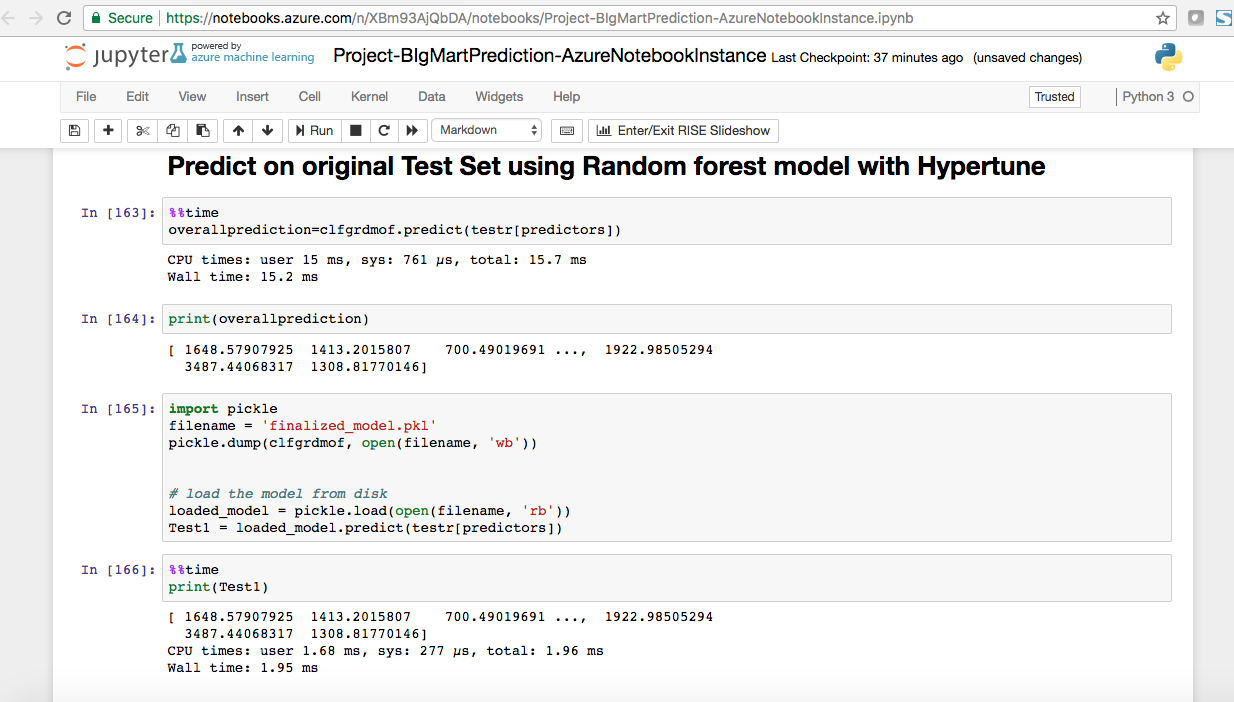
\includegraphics[width=\columnwidth]{Images/Azurenotebookscreenshot.png}
\caption{Azurenotebookscreensho}
\label{fig:Azurenotebookscreensho}
\end{figure}

\section{AWS with Notebook Instance}

On AWS SageMaker service, it can support Machine learning notebook creation 
and train the model, and do the prediction for from the fitted model. For this 
project, the Jupyter notebook instance was used for training model and 
prediction. Captured the time of execution on the same with 8.2 ms for overall 
batch prediction. With Model, the computation time is 371 micro secs.

\begin{figure}[pic10]
\centering
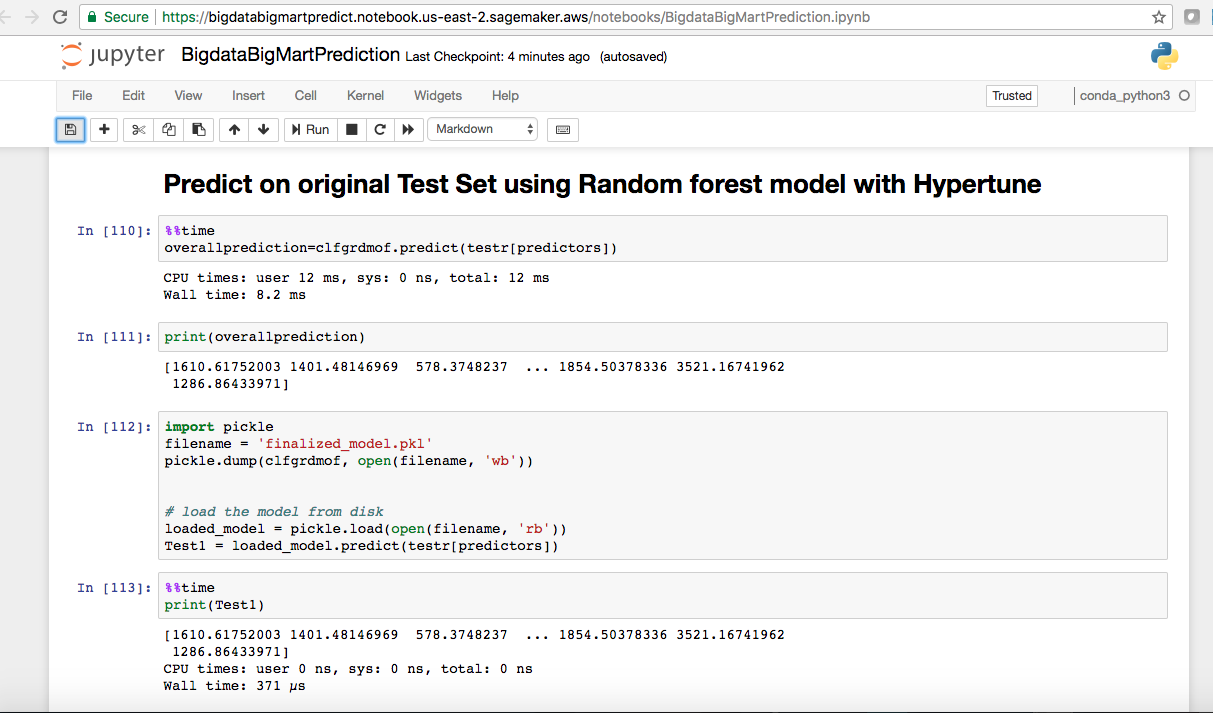
\includegraphics[width=\columnwidth]{Images/AWSnotebookscreenshot.png}
\caption{AWSnotebookscreenshot}
\label{fig:AWSnotebookscreenshot}
\end{figure}

\section{LocalMachine with Notebook Instance}

On AWS SageMaker, it can support Machine learning notebook creation and 
train the model, and do the prediction for from the fitted model. For this 
project, the Jupyter notebook instance was used for training model and 
prediction. Captured the time of execution on the same is approx 10 mins.

Start time
\begin{figure}[pic11]
\centering
\includegraphics[width=\columnwidth]{Images/Starttime_local.png}
\caption{Starttime_local}\label{fig:Starttime_local}
\end{figure}

Endtime 
\begin{figure}[pic12]
\centering
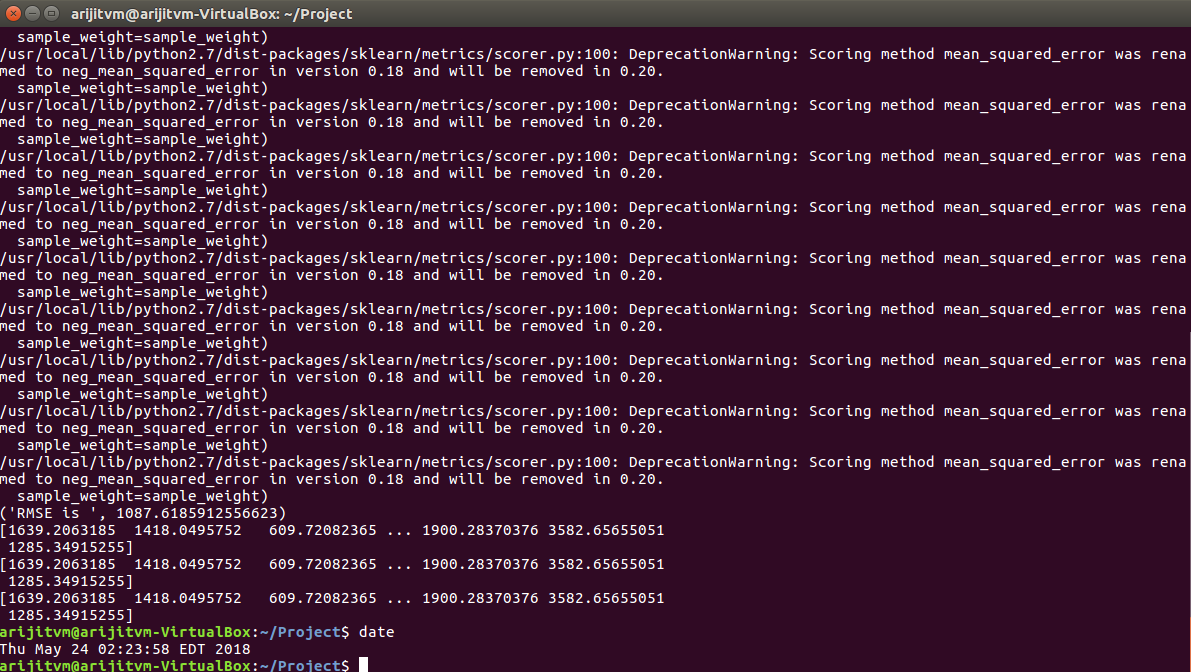
\includegraphics[width=\columnwidth]{Images/EndTime_local.png}
\caption{EndTime_local}\label{fig:EndTime_local}
\end{figure}

\section{Docker}

The Docker Image has been locally created and have shown the predicted 
price for a set of data. This can be replicated using Docker commands. 
Once replicated locally, running the locahost website will be created 
with port- 8080 exposed, will display the Bulk prediction results.
Link for localhost at http://localhost:8080/cloudmesh/prediction

\section{Conclusion}

In this project, below two models have been implemented and 
hyper-tuned in Azure ML Studio, Once we have the better model, used for 
prediction on Item Outlet Sales price for all the Items 
across all the store outlets.
\begin{itemize}
\item Boosted Decision
\item Linear Regression
\item HyperTuned Boosted Decision
\end{itemize}
Web service has been deployed on Azure Cloud, AWS Cloud, Local machine 
and Docker image and exposes 
as to generate the prediction for Item Identifiers. It seems with above 
calculation, AWS with is executing faster then Azure and local machine.

\section{Appendix}

Web service has been deployed on Azure Cloud and exposes as to generate 
the prediction for Item Identifiers.
Video recording has been uploaded at this location at
https://www.youtube.com/watch?v=xrLto4XPn1o


\begin{acks}

  The authors would like to thank Dr.~Gregor~von~Laszewski for his
  support and suggestions to write this paper.

\end{acks}

\bibliographystyle{ACM-Reference-Format}
\bibliography{report} 
